% !TeX root = ../main.tex
% Add the above to each chapter to make compiling the PDF easier in some editors.

\chapter{Experiments}\label{chapter:experiments}

\section{Datasets}
We train and test proposed skeletonization method on three datasets.

\begin{itemize}
	\item \textbf{SNEMI3D} (\cite{SNEMI3D})- Originally a segmentation challenge organized to advance and compare automatic segmentation methods, has been used a benchmark for most automatic segmentation methods. As part of the challenge, a EM image of an adult mouse brain of size $100*1024*1024$ with a resolution of $6x6x30$ nanometer was manually annotated and released. The proposed method here requires skeletons for training, so thinning based skeletonization is applied on the ground truth segmentation to obtain skeletons. For test and validation a in-house manually labeled chunk from the same dataset \cite{Kasthuri2015}, of which SNEMI3D's dataset is part-of, is used.
	\item P7 - An in-house dataset of parallel fiber \textcolor{red}{Ask donglai about details}
\end{itemize}

\subsection{Evaluation Metric}
Previous 2D skeletonization methods \cite{Wang2019}, \cite{Xu2019} were agnostic of skeleton instances, so, the error metrics - Precision and Recall - were based on direct pixelwise calculation of true positive (TP), false positive (FP) and false negative (FN). 
In current proposed method skeletons for each segment are identified separately. This demands, first matching each proposed skeleton to a ground truth skeleton, similar to error metric proposed in \cite{Liang2019}, which predicts road boundaries. Predicted skeletons are matched to one and only one ground truth skeleton instance based on its maximum overlap. Some predicted skeletons may not be matched to any ground truth, and vice versa. Precision and recall is then calculated, similar to \cite{Liang2019}, all predicted skeleton voxels within a threshold distance to ground truth skeleton is classified as TP, and rest as FP. FN are the voxels not in range of skeleton voxels. F1 score, harmonic mean of Precision and Recall is also reported.

To assess if predicted skeletons are over-split, a connectivity score is also calculated similar to \cite{Liang2019}.


\begin{figure}[htpb]
	\centering
	\begin{subfigure}[b]{0.3\textwidth}
		\centering
		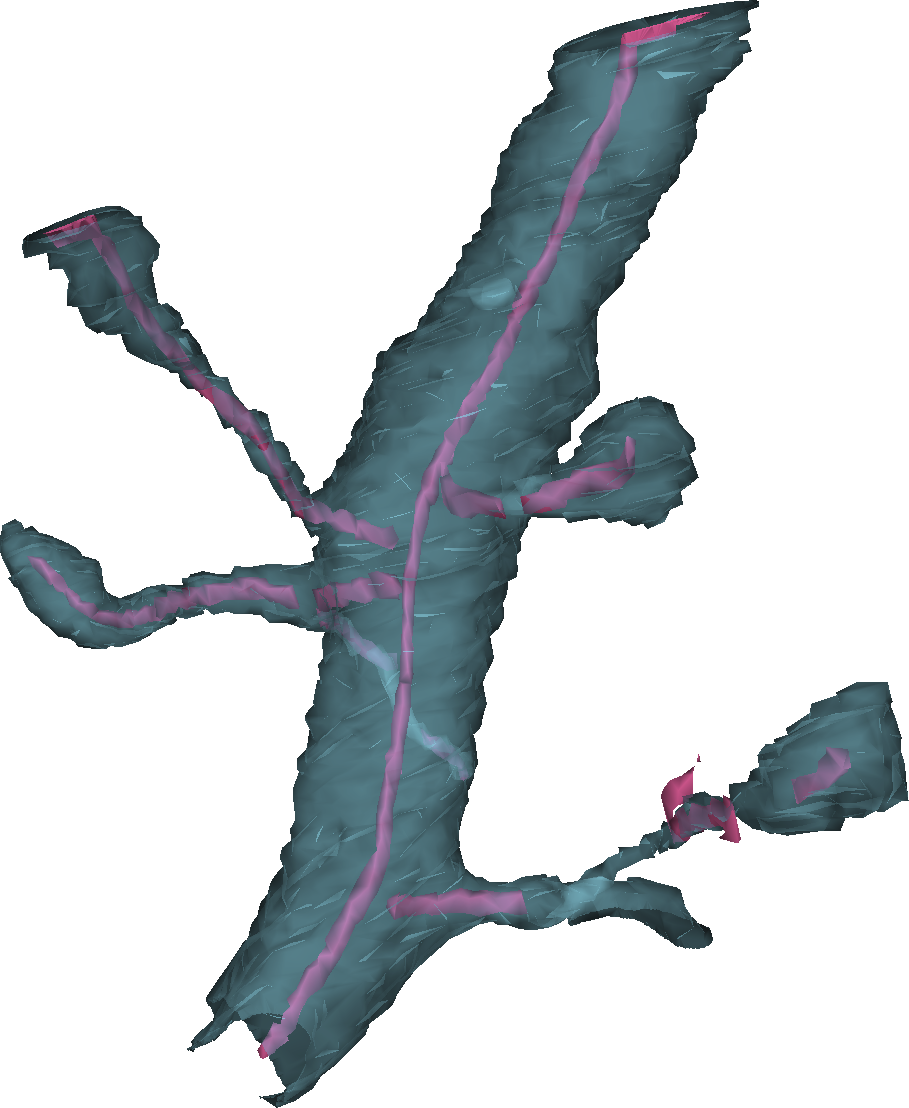
\includegraphics[width=\textwidth]{data/images/splitNMatch2/train_good.png}
		\caption{\label{fig:merged_train}}
	\end{subfigure}
	\hspace{3mm}
	\begin{subfigure}[b]{0.4\textwidth}
		\centering
		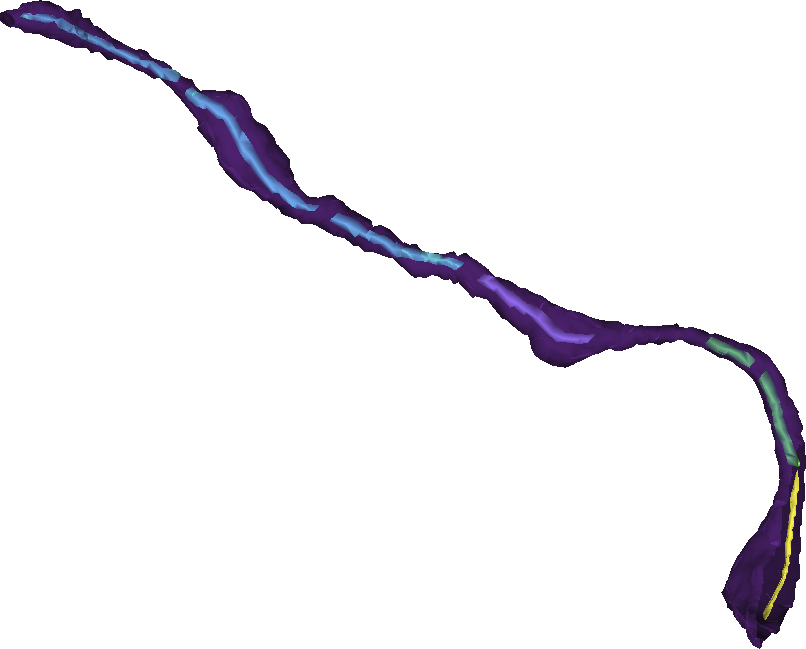
\includegraphics[width=\textwidth]{data/images/splitNMatch2/val_good_bad.png}
		\caption{\label{fig:merged_val}}
	\end{subfigure}	
	\caption{Mathching results from \subref{fig:merged_train} train and \subref{fig:merged_val} test sets of SNEMI. While \subref{fig:merged_train} shows all the skeleton parts for a segment were matched properly, \subref{fig:merged_val} shows some correctly matched and some un-matched parts}  
	\label{fig:matchedSNEMI}
\end{figure}

\begin{table*}[!ht]                                                                                          
	\centering
	\begin{adjustbox}{width=\textwidth,center=\textwidth}
	\begin{tabular}{|c|c|c|c|c|c|c|c|c|c|c|c|c|c|}                                                                      
		\hline                                                                                               
		\multirow{2}{*}{Dataset} & \multirow{2}{*}{Subset} & \multicolumn{4}{c|}{Initial}  & \multicolumn{4}{c|}{After split}  & \multicolumn{4}{c|}{After match} \\                                    
		\cline{3-14}                                                                                                  
		&  & P & R & F & C & P & R & F & C & P & R & F & C \\                                                           
		\hline                                                                                                  
		\hline                                                                                                  
				& Train & 0.64 & 0.89 & 0.74 & 0.93 & 0.66 & 0.96 & 0.78 & 0.74 & 0.66 & 0.95 & 0.78  & 0.79\\                           
		SNEMI 	& Val 	& 0.64 & 0.64 & 0.64 & 0.88 & 0.63 & 0.82 & 0.71 & 0.73 & 0.62 & 0.76 & 0.68 & 0.77 \\           
				& Test 	&  &  &  &  &  &  &  &  &  &  &  & \\
		\hline		 
				& Train &  &  &  &  &  &  &  &  &  &  &  & \\                           
		P7 		& Val 	&  &  &  &  &  &  &  &  &  &  &  & \\           
				& Test 	&  &  &  &  &  &  &  &  &  &  &  & \\                          
		\hline                                                                                                     
	\end{tabular}
	\end{adjustbox}                                                
	\caption{Skeleton prediction scores after every step. P, R, F, C stands for Precision, Recall, F-Score and Connectivity Scores.}
	\label{tab:dissected_scores}                                                                   
\end{table*}
